\documentclass[12pt, a4paper]{article}
\usepackage[a4paper, includeheadfoot, mag=1000,
            left=2cm, right=1.5cm, top=1.5cm, bottom=1.5cm,
            headsep=0.8cm, footskip=0.8cm]{geometry}
% Fonts
\usepackage{fontspec, unicode-math}
\setmainfont[Ligatures=TeX]{CMU Serif}
\setmonofont{CMU Typewriter Text}
\usepackage[english, russian]{babel}
% Indent first paragraph
\usepackage{indentfirst}
\setlength{\parskip}{5pt}
% Diagrams
\usepackage{graphicx}
\usepackage{floatrow}
% Python
\usepackage{pythontex}

\begin{document}
\begin{titlepage}

\noindent\textsc{ФГАОУ ВО «Санкт-Петербургский национальный исследовательский
университет информационных технологий, механики и оптики»\\[4mm]
Кафедра физики}
\vfill
\noindent\textbf{РАБОЧИЙ ПРОТОКОЛ И ОТЧЕТ\\[2mm]
ПО ЛАБОРАТОРНОЙ РАБОТЕ №4\\[4mm]
Изучение свойств ферромагнетика}\\[16mm]
Преподаватель Ефремова Екатерина Александровна\\[2mm]
Студенты Лабушев Тимофей Михайлович, Нестеров Дали Константинович\\[2mm]
Группа P3202
\vfill
\noindent Санкт-Петербург\\[2mm]
2018 г.

\end{titlepage}

\section*{Введение}

\subsection*{Цель работы}

Исследование петли гистерезиса, кривой первоначальной намагниченности
и графика магнитной проницаемости ферромагнетика.

\subsection*{Объект исследования}

Ферромагнетик

\subsection*{Метод экспериментального исследования}

Прямые и косвенные измерения, графическое отображение

\subsection*{Требуемое оборудование и материалы}

\begin{enumerate}
\item Генератор напряжений ГН1
\item Осциллограф ОЦЛ2
\item Стенд с объектом исследования
\item Проводники Ш4/Ш4 (2 шт), 2Ш4/BNC (2 шт)
\end{enumerate}

\subsection*{Рабочие формулы и исходные формулы}

Ферромагнитный материал ниже точки Кюри находится в так называемом
магнитоупорядоченном состоянии: весь объем образца разбивается на области,
в каждой из которых атомные магнитные моменты ориентированы в
одинаковом направлении. Эти области, размеры которых заметно превосходят
межатомные расстояния, называются \textit{ферромагнитными доменами}.
Магнитные свойства ферромагнетика определяется перестройкой его доменной
структуры (прежде всего смещением границ доменов) под действием внешнего
магнитного поля. Характер изменения магнитной индукции $B$ в зависимости от
напряженности $H$ магнитного поля внутри типичного ферромагнетика показан
на рисунке 1. Если к первоначально ненамагниченному образцу прикладывать
усиливающееся внешнее магнитное поле, то магнитная индукция изменяется в
соответствии с кривой первоначального намагничивания $abc$. На начальном
участке этой кривой магнитная индукция быстро и нелинейно возрастает с
ростом магнитной напряженности. Затем в некоторой точке ($H_s$, $B_s$) рост
функции $B(H)$ сильно замедляется и становится линейным. Этот второй участок
графика (он не изображен на рис.1) называется \textit{областью насыщения
намагниченности}. Если же после достижения некоторого значения
напряженности, например, $H_m$, в точке $b$ начать уменьшать напряженность, то
намагниченность образца и магнитная индукция внутри него уменьшаются с
некоторым запаздыванием, не обращаясь в ноль при $H = 0$. Такое запаздывание
называется \textit{гистерезисом}. Петля, которую описывает точка, изображающая
состояние образца в координатах ($H$, $B$) при периодическом изменении
магнитной напряженности, называется \textit{петлей гистерезиса}. На рисунке 1
изображены две таких петли, одна – для колебаний напряженности с
амплитудой $H_m$, другая – для колебаний с амплитудой $H_s$.

\begin{figure}[H]
\floatbox[{\capbeside\thisfloatsetup{capbesideposition={right,top},capbesidewidth=4cm}}]{figure}[\FBwidth]
{\caption{Зависимость магнитной индукции от напряженности магнитного поля в ферромагнетике. Петля гистерезиса}}
{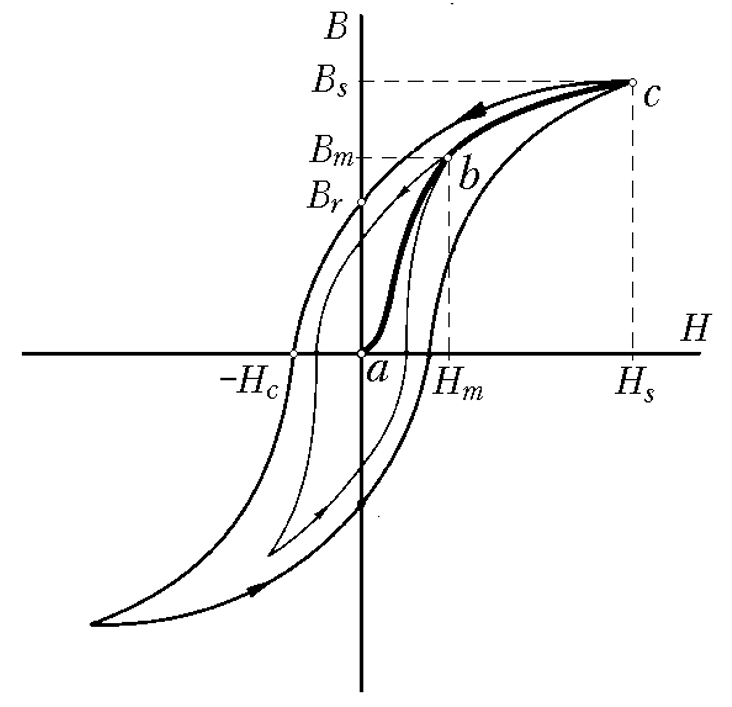
\includegraphics[width=0.35\textwidth]{lab4.png}}
\end{figure}

Важными характеристиками ферромагнетика являются остаточная магнитная индукция $B_r$
и коэрцитивная сила $H_c$. Магнитная проницаемость ферромагнетика $\mu$ определяется
следующим соотношением:
\begin{equation}
\mu = \frac{1}{\mu_0}\frac{B_m}{H_m}
\end{equation}
где $\mu_0 = 4\pi \cdot 10^{-7}$ Гн/м – магнитная постоянная; $B_m$, $H_m$ —
индукция и напряженность магнитного поля в магнетике, соответствующие кривой
начального намагничивания. Кривая начального намагничивания строится по
вершинам петель гистерезиса с разным максимальным значением магнитной
напряженности $H_m$.

В качестве образца для изучения магнитных свойств ферромагнитного
материала выбран сердечник трансформатора, размещенного на лабораторном
стенде (см. рис.2). Мгновенная напряженность $Н$ магнитного поля,
создаваемого первичной обмоткой в образце, отображается по горизонтальной
оси осциллографа:
\begin{equation}
H = \alpha X,\ \alpha = \frac{K_X N_1}{l R_1}
\end{equation}
где $X$ — координата луча по горизонтальной оси ОХ экрана осциллографа при условии,
что начало координат находится в центре петли гистерезиса; $K_X$ (В/дел) – масштаб
развертки по оси ОХ; $N_1$ – число витков первичной обмотки; $l$ – длина
средней линии сердечника, на котором равномерно распределена первичная обмотка;
$R_1$ – сопротивление соединенного последовательно с первичной обмоткой резистора.

\begin{figure}[H]
\floatbox[{\capbeside\thisfloatsetup{capbesideposition={right,top},capbesidewidth=4cm}}]{figure}[\FBwidth]
{\caption{Электрическая схема подключения стенда для изучения магнитных свойств материала.
Исследуемым образцом служит сердечник трансформатора}}
{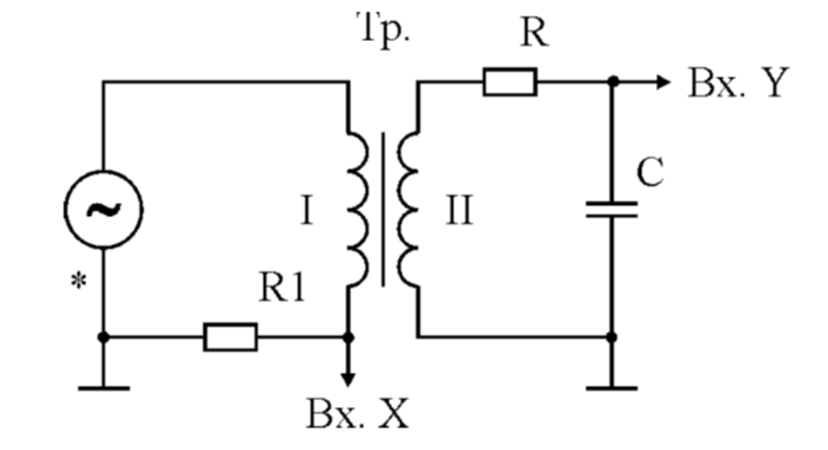
\includegraphics[width=0.5\textwidth]{lab4_2.png}}
\end{figure}

Мгновенное значение индукции $B$ магнитного поля в образце отображается
по вертикальной оси экрана осциллографа:
\begin{equation}
B = \beta Y,\ \beta = \frac{K_Y RC}{N_2 S}
\end{equation}
где $K_Y$ (B/дел) – масштаб развертки по оси ОY; $R$ и $С$ –
сопротивление и емкость, подключенные ко вторичной обмотке трансформатора;
$N_2$ – число витков вторичной обмотки; $S$ – площадь
поперечного сечения сердечника.

Временнóе запаздывание магнитной индукции в образце относительно
напряженности магнитного поля приводит к потерям энергии. При этом
средняя мощность, расходуемая внешним источником тока при циклическом
перемагничивании ферромагнитного образца, пропорциональна площади $S_{hl}$
петли гистерезиса:
\begin{equation}
P = \chi S_{hl},\ \chi = K_X K_Y \frac{\nu N_1 RC}{N_2 R_1}
\end{equation}
где $\nu$ — частота колебаний напряжения, подаваемого на первичную обмотку.

\newpage
\section*{Ход работы}

\subsection*{Исходные параметры}

\begin{pycode}
import numpy as np

N_1 = 1665
N_2 = 970
L = 7.8 * 10**-2
S = 0.64 * 10**-4
R_1 = 68
R_2 = 470 * 10**3
C = 0.47 * 10**-6
freq = 40
K_X = 0.25
K_Y = 0.1
\end{pycode}

\noindent
$$N_1 = \py{N_1} \textup{ витков}, N_2 = \py{N_2} \textup{ витков},
L = \py{L * 10**2} \pm 0.1 \textup{ см}, S = \py{np.round(S * 10**4, 2)} \pm 0.05 \textup{ см}^2$$
$$R_1 = \py{R_1} \textup{ Ом} \pm 10\%, R_2 = \py{R_2} \textup{ Ом} \pm 10\%,
C = \py{C * 10**6} \textup{ мкФ} \pm 10\%$$
$$\nu = \py{freq} \pm 5 \textup{ Гц}, K_X = \py{K_X} \textup{ В}, K_Y = \py{K_Y} \textup{ В}$$

\subsection*{Параметры гистерезисной петли}

Для снятых показаний $U$, $K_X$, $К_Y$, $X$, $Y$ рассчитаем мгновенные значения
напряженности $H$ и индукции $B$ магнитного поля по формулам (2) и (3) соответственно,
на основании которых найдем магнитную проницаемость $\mu$ по формуле (1):

\begin{pycode}
import re
from tabulate import tabulate

def latex_table(data, headers):
  s = tabulate(data, headers=headers, tablefmt='latex')
  # https://github.com/gregbanks/python-tabulate/issues/5
  s = re.sub(r'(\^\{\})', "^", s); s = re.sub(r'\\([\$\_\{\}\^])', r'\1', s); s = re.sub(r'(\\textbackslash{})', r'\\', s)
  return s

data = [
  [4.5, 0.05, 0.05, 28 / 10, 9 / 10],
  [6, 0.1, 0.05, 18 / 10, 14 / 10],
  [7.5, 0.1, 0.05, 23 / 10, 19 / 10],
  [9, 0.1, 0.05, 30 / 10, 23 / 10],
  [10.5, 0.25, 0.05, 16 / 10, 28 / 10],
  [12, 0.25, 0.05, 19 / 10, 31 / 10],
  [13.5, 0.25, 0.05, 23 / 10, 35 / 10]
][::-1]

def alpha(k_x): return f'${k_x * N_1 / (R_1 * L):.3f}$'
def beta(k_y): return f'${k_y * R_2 * C / (N_2 * S):.3f}$'
def H_float(k_x, x): return x * k_x * N_1 / (R_1 * L);
def H(k_x, x): return f'${H_float(k_x, x):.3f}$'
def B_float(k_y, y): return y * k_y * R_2 * C / (N_2 * S);
def B(k_y, y): return f'${B_float(k_y, y):.4f}$'
def mu_float(k_x, x, k_y, y):
  mu_0 = 4 * np.pi * 10**-7
  return (1 / mu_0) * (B_float(k_y, y) / H_float(k_x, x))
def mu(k_x, x, k_y, y): return f'${mu_float(k_x, x, k_y, y):.3f}$'

table1 = [[u, k_x, k_y, x, y, alpha(k_x), beta(k_y), H(k_x, x), B(k_y, y), mu(k_x, x, k_y, y)] for [u, k_x, k_y, x, y] in data]
\end{pycode}

\begin{table}[H]
\py{latex_table(table1, ['$U$', '$K_X$', '$K_Y$', '$X$', '$Y$', '$\\alpha$', '$\\beta$', '$H_m$', '$B_m$', '$\\mu$'])}
\end{table}

\subsection*{Средняя мощность, расходуемая на перемагничивание}

Определим среднюю мощность $P$, затрачиваемую при циклическом перемагничивании
ферромагнитного образца по формуле (4), предварительно измерив площадь петли в
делениях шкалы осциллографа.

Перенесенное на лист измерений изображение имеет площадь $3.52 \textup{дел}^2$.

\begin{pycode}
def chi_float(): return K_X * K_Y * (freq * N_1 * R_2 * C) / (N_2 * R_1);
def chi(): return f'{chi_float():.3f}'
def P_float(): return chi_float() * 3.52;
def P(): return f'{P_float():.4f}'
\end{pycode}

$$\chi = K_X K_Y \frac{\nu N_1 R C}{N_2 R_1} = \py{chi()}, P = \chi S_{hl} = \py{P()} \textup{ Вт}$$

\subsection*{Погрешности косвенных измерений}

Основываясь на приборных погрешностях $\Delta\nu = 5 \textup{ Гц},
\Delta R_1 = 6.8 \textup{ Ом}, \Delta R_2 = 47000 \textup { Ом}, \Delta C = 0.047 \cdot 10^{-6} \textup{ Ф}$,
вычислим погрешность рассчитанного значения $P$:

$$\Delta P = P(\frac{\Delta\nu}{\nu} + \frac{\Delta R_1}{R_1} + \frac{\Delta R_2}{R_2} + \frac{\Delta C}{C}) =
\py{np.round(P_float() * (5 / freq + 6.8 / R_1 + 47000 / R_2 + (0.047 * 10**-6) / C), 4)} \textup{ Вт}$$

\subsection*{График начального намагничивания $B_m = f(H_m)$}

\begin{pycode}
import matplotlib.pyplot as plt

hb_table = [[H_float(k_x, x), B_float(k_y, y)] for [u, k_x, k_y, x, y] in data]
hs, bs = np.transpose(hb_table).tolist()
plt.figure(figsize=(7, 4))
plt.plot(hs, bs, '-o')
plt.axis((0, 190, 0, 0.7))
plt.grid()
plt.savefig('hb_plot.pdf', bbox_inches='tight')
\end{pycode}

\begin{figure}[H]
\includegraphics[width=0.65\textwidth]{hb_plot.pdf}
\end{figure}

\subsection*{График магнитной проницаемости $\mu = f(H_m)$}

\begin{pycode}
hmu_table = [[H_float(k_x, x), mu_float(k_x, x, k_y, y)]
  for [u, k_x, k_y, x, y] in data]
hs, mus = np.transpose(hmu_table).tolist()
plt.figure(figsize=(7, 4))
plt.plot(hs, mus, '-o')
plt.axis((0, 190, 0, 6000))
plt.grid()
plt.savefig('hmu_plot.pdf', bbox_inches='tight')
\end{pycode}

\begin{figure}[H]
\includegraphics[width=0.65\textwidth]{hmu_plot.pdf}
\end{figure}

\end{document}
